\chapter{Opdracht}

In 2017 heeft Quintor in samenwerking met DUO/MinOCW, Groningen Declaration Network, Stichting ePortfolio Support, TNO en Rabobank, het Blockchain Field-lab Education gestart in Groningen. Het Blockchain-lab is opgezet om expertise en kennis uit te wisselen op regionaal, nationaal en internationaal gebied. De oprichting van het Blockchain Field-lab Education heeft er mede voor gezorgd dat Quintor meer kennis wilt opdoen op het gebied van Blockchain. Daarnaast bestaat er de mogelijkheid dat het bedrijf in de toekomst Blockchain technologie wilt inzetten om vraagstukken vanuit klanten op te lossen.

\begin{figure}[h]
  \centering
  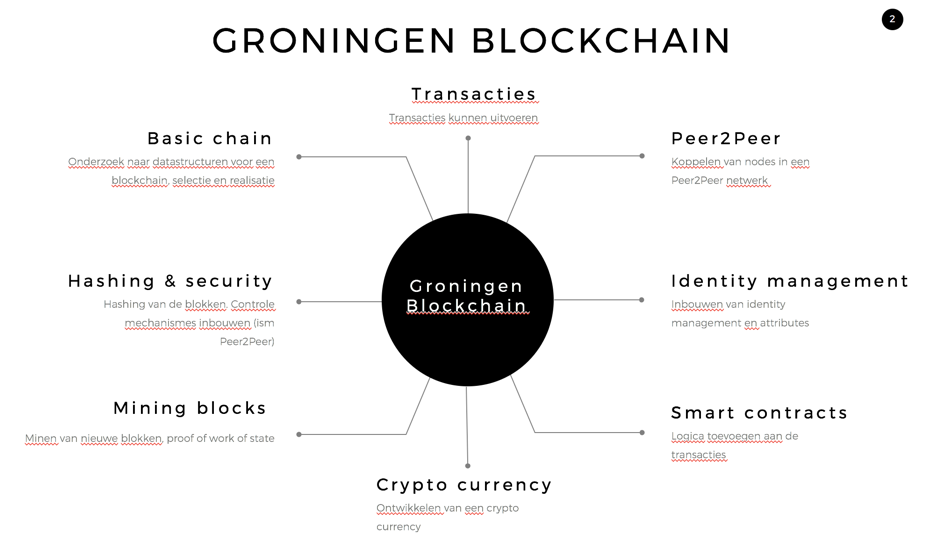
\includegraphics{figures/indeling_blockchain_opdracht}
  \caption{Indeling opdracht Blockchain ontwikkeling zoals gegeven door Quintor afkomstig uit.}
  \label{indeling_blockchain_opdracht} 
\end{figure}

De focus in de afstudeeropdracht ligt op de Blockchain onderdelen Identity Management en Peer2Peer (Distributed Network). Dit zal in samenwerking gaan met een andere afstudeerder, Kevin Bos, die verantwoordelijk is voor de onderdelen Basic chain, Hashing \& security en Mining blocks. 

\newpage
\section{Probleemstelling}

Sinds de opkomst van Bitcoin is de Blockchain technologie, de techniek die het mogelijk maakt om het op een gedecentraliseerde manier te laten werken, steeds populairder geworden. Alhoewel de Blockchain-technologie nog in de kinderschoenen staat, gaan de ontwikkelingen in het domein zeer snel. Zo worden er toepassingen bedacht die niet alleen voor de financiële markten interessant zijn, maar ook voor bijvoorbeeld het digitaliseren van contracten en contractbeheer.

Aangezien de toepassing en adoptie van Blockchain technologie steeds groter wordt wil Quintor de toepassingsmogelijkheden en technieken onderzoeken om zo inzicht te kunnen krijgen in hoe het gebruikt kan worden in de aangeboden vraagstukken vanuit klanten.

\section{Doelstelling}

De doelstelling van de opdracht is verspreid over onderdelen van Blockchain technologie, zoals te zien in fig. \ref{indeling_blockchain_opdracht}. Hierdoor is er een globaal doel en een doel die specifiek voor deze opdracht geldt. Het streven naar het globale doel is het opdoen van kennis omtrent het realiseren van een Blockchain implementatie. Het doel van deze specifieke opdracht is middels het opstellen van een proof-of-concept van de Blockchain onderdelen Identity Management en Distributed Network, zonder gebruik te maken van bestaande Blockchain protocollen, kennis te ontwikkelen voor Quintor op het gebied van Blockchain technologie.

\section{Resultaat}

Indien de opdracht succesvol afgerond is, zijn de onderdelen Identity Management en het Peer2Peer netwerk gerealiseerd aan de hand van voorgestelde technieken die voortgekomen zijn uit het gedane onderzoek. In samenwerking met de onderdelen die gerealiseerd zijn door Kevin Bos zal er een werkend Proof of Concept van een Blockchain gerealiseerd zijn. Zowel het Proof of Concept als het onderzoek zal voor Quintor inzicht bieden in het Blockchain domein en de ontwikkelingen daarin.

\subsection{Producten}

Als onderdeel van de afstudeeropdracht zullen er verschillende producten worden opgeleverd aan Quintor en aan de Haagse Hogeschool. Deze staan hieronder gespecificeerd.

De op te leveren producten aan Quintor zijn:
\begin{itemize}
  \item{Adviesrapport}
  \item{Sprint demo presentaties}
  \item{Broncode van de ontwikkelde applicatie}
  \item{Opgestelde documentatie}
\end{itemize}

De op te leveren producten aan de Haagse Hogeschool zijn:
\begin{itemize}
  \item{Afstudeerscriptie}
  \item{Plan van Aanpak}
  \item{Adviesrapport}
  \item{Testrapport}
  \item{Technisch ontwerp}
\end{itemize}


